\documentclass{standalone}
\usepackage{tikz}

\begin{document}

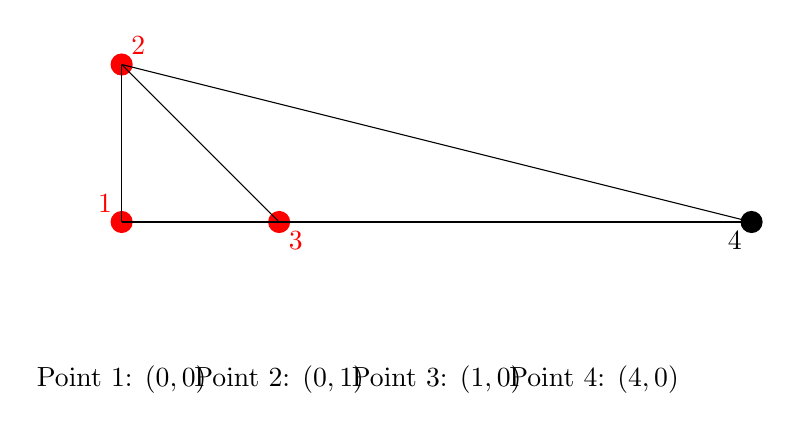
\begin{tikzpicture}[scale=2]
    % Define the coordinates
    \coordinate (A) at (0,0);
    \coordinate (B) at (0,1);
    \coordinate (C) at (1,0);
    \coordinate (D) at (4,0);

    % Draw the points
    \fill[red] (A) circle (2pt) node[above left] {1};
    \fill[red] (B) circle (2pt) node[above right] {2};
    \fill[red] (C) circle (2pt) node[below right] {3};
    \fill (D) circle (2pt) node[below left] {4};

    % Draw lines connecting the points
    \draw (A) -- (B);
    \draw (B) -- (C);
    \draw (C) -- (A);
    \draw (A) -- (D);
    \draw (B) -- (D);
    \draw (C) -- (D);

    % Label the points
    \node at (0,-1) {Point 1: $(0,0)$};
    \node at (1,-1) {Point 2: $(0,1)$};
    \node at (2,-1) {Point 3: $(1,0)$};
    \node at (3,-1) {Point 4: $(4,0)$};

\end{tikzpicture}

\end{document}